\documentclass[a4paper,12pt]{article}
\usepackage[utf8]{inputenc}
\usepackage[russian]{babel}
\usepackage{amsmath}
\usepackage{amssymb}
\usepackage{enumitem}
\usepackage{emoji}
\usepackage{graphicx}
\usepackage[a4paper, top= 1cm, bottom=2cm, left=2cm, right=2cm]{geometry}

\title{Оценка + пример}


\begin{document}
\maketitle

\subsection*{Что это такое и с чем его едят?}
Иногда в задачах нужно доказательство с двух сторон. Например, если просят доказать, что ответ именно такой, нужно доказать, что он не может быть меньше и не может быть больше (и при этом он может быть равным) - это и называется оценкой с двух сторон. В предложенных задачах нужно не только доказать оценку, но и показать, что данный ответ подходит, предъявив пример. Давайте разберёмся, как это применяется в жизни...

    \subsection*{Попробуем понять на простом примере}
        \subsubsection*{Задача}
            Какое наибольшее число трёхклеточных уголков можно вырезать из клетчатого квадрата 8 × 8?
        
        \subsubsection*{Решение} 
            \underline{Оценка:} В квадрате 64 клетки. Поэтому вырезать 22 и более уголков не получится: ведь тогда суммарное число клеток в них будет не меньше 22 · 3 = 66. Значит, число уголков не больше 21. 
            \underline{Пример:} Вырезать 21 уголок можно, пример приведён на рисунке.
                \begin{figure}[h]
                    \centering
                    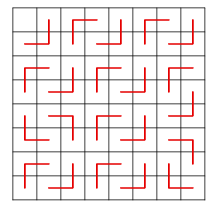
\includegraphics[width=0.35\linewidth]{example.png}
                    \caption{Пример вырезанных уголков}
                    \label{fig:corner-example}
                \end{figure}

\subsection*{Задачи}
    \begin{enumerate}
        \item Какое наибольшее количество ладей можно расставить на доске $10 \times 10$, чтобы они не били друг друга?
        \item Какое наименьшее число ладей могут побить всю шахматную доску?
        \item Какое наименьшее количество клеток на шахматной доске надо отметить, чтобы в любом квадратике 2x2 нашлась хотя бы одна отмеченная клетка?
        \item Каким наименьшим числом монет в 3 и 5 копеек можно набрать сумму 37 копеек? 
        \item Белоснежка вошла в комнату, где вокруг круглого стола стояло 30 стульев. На некоторых из стульев сидели гномы. Оказалось, что Белоснежка не может сесть так, чтобы рядом с ней никто не сидел. Какое наименьшее число гномов могло быть за столом? (Объясните, как должны были сидеть гномы и почему, если бы гномов было меньше, Белоснежка нашла бы стул, рядом с которым никто не сидит).
        \item Электронные часы показывают время в стандартном формате (например, 20:27). Найдите наибольшее возможное значение произведения цифр на таких часах.
        \item Какое наименьшее число клеток на доске 8×8 можно закрасить так, чтобы была хотя бы одна закрашенная клетка в любом уголке из трёх клеток?
        \item Двенадцать стульев стоят в ряд. Иногда на один из свободных стульев садится человек. При этом ровно один из его соседей (если они были) встаёт и уходит. Какое наибольшее количество человек могут одновременно оказаться сидящими, если вначале все стулья были пустыми?
    \end{enumerate}
\end{document}
